\documentclass[twoside,10pt]{book} 
\usepackage{graphicx}
\usepackage{color}
\usepackage{graphics}
\usepackage{listings}
\usepackage{natbib}
\usepackage{fullpage}
\usepackage{amssymb}
\usepackage{verbatimfiles}
\usepackage[dvips]{hyperref}
\begin{document}
\lstset{
  language=Python,
  basicstyle=\scriptsize,
  commentstyle=\color{blue},
  stringstyle=\ttfamily,
  showstringspaces=false,
%  frame=single, 
  breaklines=true,
  breakatwhitespace = true,
  postbreak = \space\dots
}


\newcommand{\fig}[4]
{\begin{figure}[ht]
\begin{center}
\includegraphics[width=#1]{#2}
\caption{\label{#4} #3}
\end{center}
\end{figure}}

\newcommand{\mytextsize}[0]{\footnotesize}
\newcommand{\myheadersize}[0]{\small}
\newcommand{\matlab}[0]{matlab{\texttrademark}}
\newcommand{\fname}[1]{{\tt #1}}
\newcommand{\func}[1]{{\tt #1}}
\newcommand{\code}[1]{{\tt #1}}
\newcommand{\prompt}[1]{\code{>>> #1}}
\newcommand{\carg}[1]{\textit{#1}} % command argument
\newcommand{\val}[1]{\textit{#1}}
\newcommand{\rc}[1]{{\tt #1}}

% a pointer to matplotlib documentation
\newcommand{\mpldoc}[1]{#1}
%\newcommand{\url}[1]{{\tt #1}}

\mytextsize
\section*{\large The Matplotlib Hacking Points Memo \normalsize by John D. Hunter}

matplotlib is a library for making 2D plots of arrays in
python.\footnote{This short guide is not meant as a complete guide or
  tutorial, but rather introduces a few features of matplotlib.
  Please see the examples directory of the matplotlib source
  distribution for many more examples, the tutorial on the web page,
  and the soon to be released user's guide, which aims to be
  comprehensive!  } Although it has its origins in emulating the
\matlab\ graphics commands, it does not require matlab, and has a
pure, object oriented API.  Although matplotlib is written primarily
in pure python, it makes heavy use of Numeric/numarray and other
extension code to provide good performance even for large arrays.

matplotlib is designed with the philosophy that you should be able to
create simple plots with just a few commands, or just one!  If you
want to see a histogram of your data, you shouldn't need to
instantiate objects, call methods, set properties, and so it; it
should just work.  

The matplotlib code is divided into three parts: the \textit{matlab
  interface} is the set of functions provided by matplotlib.matlab
which allow the user to create plots with code quite similar to matlab
figure generating code.  The \textit{matplotlib frontend} or
\textit{matplotlib API} is the set of classes that do the heavy
lifting, creating and managing figures, text, lines, plots and so on.
This is an abstract interface that knowns nothing about output.  The
\textit{backends} are device dependent drawing devices, aka renderers,
that transform the frontend representation to hardcopy or a display
device.  Example backends: PS creates postscript hardcopy, SVG creates
scalar vector graphics hardcopy, Agg creates PNG output using the high
quality antigrain library that ships with matplotlib -
\url{http://antigrain.com}, GTK embeds matplotlib in a GTK
application, GTKAgg uses the antigrain renderer to create a figure and
embed it a GTK application, and so on for WX, Tkinter, FLTK\dots.



\section*{\myheadersize Migrating from \matlab}

Using matplotlib should come naturally if you have ever plotted with
matlab, and should be fairly straightforward if you haven't.  Like all
interpreted languages used for serious number crunching, python has an
extension module for processing numeric arrays.  Numerical python has
been around since the early days, and already comes with many matlab
compatible analysis functions, which matplotlib extends.  The example
code below shows two complete scripts: on the left hand side is python
with matplotlib, and on the right is matlab.  

Both scripts do the same thing: generate a white noise vector,
convolve it with an exponential function, add it to a sine wave, plot
the signal in one subplot and plot the power spectrum in another.

\begin{table}[htbp]
  \centering
  \begin{tabular}[t]{l|ll}
\begin{lstlisting}
# python                           
from matplotlib.matlab import *    

dt = 0.01                          
t = arange(0,10,dt)                
nse = randn(len(t))                
r = exp(-t/0.05)                   

cnse = conv(nse, r)*dt             
cnse = cnse[:len(t)]               
s = 0.1*sin(2*pi*t) + cnse         

subplot(211)                       
plot(t,s)                          
subplot(212)                       
psd(s, 512, 1/dt)                  
\end{lstlisting}&

\begin{lstlisting}
% matlab
% no import necessary

dt = 0.01;
t = [0:dt:10];
nse = randn(size(t));
r = exp(-t/0.05);

cnse = conv(nse, r)*dt;
cnse = cnse(1:length(t));
s = 0.1*sin(2*pi*t) + cnse;

subplot(211)
plot(t,s)
subplot(212)
psd(s, 512, 1/dt)
\end{lstlisting}&

\raisebox{-15ex}{
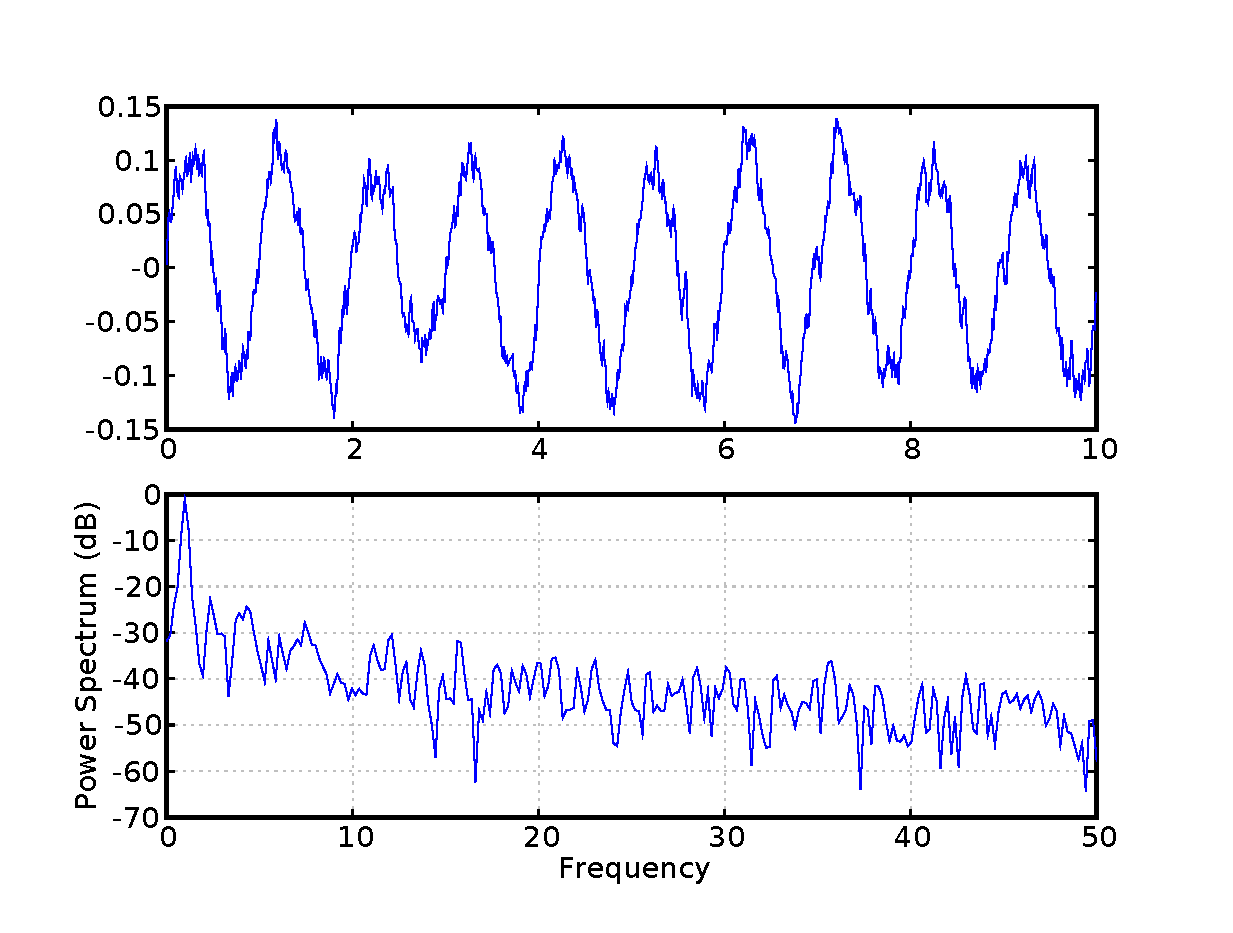
\includegraphics[width=2.3in]{figures/psd_py}}\\

\end{tabular}
\end{table}

The major differences are 1) Numeric has a functions for creating
arrays (\func{arange} above) whereas matlab has the handy notation
\code{[0:dt:10]}, 2) python uses square brackets rather than
parentheses for array indexing, and there are some small differences
in how do array lengths, sizes, and indexing.  But the differences are
minute compared to the similarities: 1) matlab and Numeric both do
array processing and have a variety of functions that efficiently
operate on arrays and scalars, 2) moderately sophisticated signal
processing (white noise, convolution, power spectra) is achieved in
only a few lines of clear code and 3) plots are simple, intuitive and
attractive.

\section*{\myheadersize Numerix}
Currently, Numeric and numarray have different strength.
Performance-wise, Numeric is faster for smallish arrays and numarray
for largish arrays.  Thus for the near-term, members of the python
community will utilize both.  Several numarray/Numeric developers are
codevelopers of matplotlib, giving matplotlib full Numeric and
numarray compatibility, thanks in large part to Todd Miller's
matplotlib.numerix module and the numarray compatibility layer for
extension code.  

One difficulty confronting users who need to work with both Numeric
and numarray is the different organizations of the two packags

\begin{lstlisting}
# Numeric                              # numarray
from Numeric import array, where       from numarray import array, where
from MLab import mean, std             from numarray.linear_algebra.mlab  import mean, std
from Numeric import convolve           from numarray.convolve import convolve
from FFT import fft                    from numarray.fft import fft
\end{lstlisting}

\noindent The matplotlib.numerix module imports all the names from these
packages into a single namespace, allowing you to do

\begin{lstlisting}
from matplotlib.numerix import array, where, convolve, mean, fft
\end{lstlisting}

\noindent The actual symbols that are imported (Numeric's or
For the remainder of this manual, the term \textit{numerix} is used to
mean either the Numeric or numarray package.  You can either package
from the prompt with

\begin{lstlisting}
  > python myscript.py --numarray  # use numarray
  > python myscript.py --Numeric   # use Numeric
\end{lstlisting}


\noindent Typically, however, users will choose one or the other and
make this setting in their matplotlib configuration file.

\noindent \textit{CAVEAT}: If your NUMERIX compile time setting and numerix rc
file setting do not agree, your performance can suffer 10-fold.
Before compiling matplotlib, edit \fname{setup.py} and
\fname{.matplotlibrc} to make sure these settings agree.  If you are
using a precompiled version of matplotlib, eg a windows installer,
make sure you choose the installer that agrees with the array package
you use most.  The installer labelled 'numarray' is for numarray
users, whereas the unlabelled installer is for Numeric users.

\section*{\myheadersize Using mathtext}

\begin{table}[htbp]
  \centering
  \begin{tabular}[t]{ll}
\lstinputlisting[lastline=32]{code/integral_demo.py}   &
\raisebox{-15ex}{
\includegraphics[width=2.5in]{figures/integral_demo}}
  \end{tabular}
  \caption{Using custom polygons and mathtext.}
\end{table}

Any text element can use math text.  You need to use raw strings
(precede the quotes with an \code{r}), and surround the string text
with dollar signs, as in \TeX.
\begin{lstlisting}
# plain text             # math text
title('alpha > beta')    title(r'$\alpha > \beta$')
\end{lstlisting}
You can also use a large number of the \TeX\ symbols\footnote{The following \TeX\ symbols are
supported: {\tiny Delta Downarrow Gamma Im LEFTangle LEFTbrace
  LEFTbracket LEFTparen Lambda Leftarrow Leftbrace Leftbracket
  Leftparen Leftrightarrow Omega P Phi Pi Psi RIGHTangle RIGHTbrace
  RIGHTbracket RIGHTparen Re Rightarrow Rightbrace Rightbracket
  Rightparen S SQRT Sigma Sqrt Theta Uparrow Updownarrow Upsilon Vert
  Xi aleph alpha approx angstrom ast asymp backslash beta bigcap
  bigcirc bigcup bigodot bigoplus bigotimes bigtriangledown
  bigtriangleup biguplus bigvee bigwedge bot bullet cap cdot chi circ
  clubsuit coprod cup dag dashv ddag delta diamond diamondsuit div
  downarrow ell emptyset epsilon equiv eta exists flat forall frown
  gamma geq gg heartsuit hspace imath in infty int iota jmath kappa
  lambda langle lbrace lceil leftangle leftarrow leftbrace leftbracket
  leftharpoondown leftharpoonup leftparen leftrightarrow leq lfloor ll
  mid mp mu nabla natural nearrow neg ni nu nwarrow odot oint omega
  ominus oplus oslash otimes phi pi pm prec preceq prime prod propto
  psi rangle rbrace rceil rfloor rho rightangle rightarrow rightbrace
  rightbracket rightharpoondown rightharpoonup rightparen searrow
  sharp sigma sim simeq slash smilespadesuit sqcap sqcup sqrt
  sqsubseteq sqsupseteq subset subseteq succ succeq sum supset
  supseteq swarrow tau theta times top triangleleft triangleright
  uparrow updownarrow uplus upsilon varepsilon varphi varphi varrho
  varsigma vartheta vdash vee wedge wp wr xi zeta}.}, as in
$\mathtt{\backslash infty}$, $\mathtt{\backslash leftarrow}$,
$\mathtt{\backslash sum}$, $\mathtt{\backslash int}$; see mathtext
module documentation for a complete list.  The over/under
subscript/superscript style is also supported.  To write the sum of
$x_i$ from 0 to infinity ($\sum_{i=0}^\infty x_i$), you could do
\begin{lstlisting}
  text(1, -0.6, r'$\sum_{i=0}^\infty x_i$')
\end{lstlisting}
The default font is \textit{italics} for mathematical symbols.  To
change fonts, eg, to write 'sin' in a \textrm{roman font}, enclose the
text in a font command, as in
\begin{lstlisting}
text(1,2, r's(t) = $\cal{A}\rm{sin}(2 \omega t)$')
\end{lstlisting}


\noindent Fairly complex \TeX\ expressions render correctly; for example, 
\begin{lstlisting}
r'$\cal{R}\prod_{i=\alpha}^\infty a_i\rm{sin}(2 \pi f x_i)$'
\end{lstlisting}
which is rendered by \TeX\ as $\mathcal{R}\prod_{i=\alpha}^\infty
a_i\mathrm{sin}(2 \pi f x_i)$.  

The mathtext module is released under the matplotlib license (PSF
compatible).  The \textit{fonts} it currently uses are the Bakoma
computer modern truetype fonts, which are free only for non-commercial
use.  It would not be too difficult to plug in a different set of
fonts which do not have these licensing restrictins, though this has
not been implemented yet.  See the mathtext module documentation for
the licensing restrictions of the Bakoma fonts.

\section*{\myheadersize Images}

matplotlib provides support for working with raw image data in numerix
arrays; currently, there is support for \textit{loading image data}
only from PNG files and other formats are on the TODO list.  The
following examples will assume you have your image data loaded into a
numerix array, either luminance (MxN), RGB (MxNx3) or RGBA (MxNx4).

An axes image is created with \code{im = imshow(X)} where \carg{X} is
a numerix array an \carg{im} is a \mpldoc{matplotlib.image.AxesImage}
instance.  The image is rescaled to fit into the current axes box.
There are two parameters that determine how the image is resampled
into the axes bounding box: \carg{interpolation} and \carg{aspect}.
The following \carg{interpolation} schemes are available:
\val{bicubic, bilinear, blackman100, blackman256, blackman64, nearest,
  sinc144, sinc256, sinc64, spline16, and spline36}.  The default
interpolation method is given by the value of \rc{image.interpolation}
in your \fname{.matplotlibrc} file.  \carg{aspect} can be either
\val{preserve} or \val{free} which will constrain the aspect ratio of
the image or not, respectively.  The default aspect setting is given
by the value of the rc parameter \rc{image.aspect}.

The full syntax of the \func{imshow} command is
\begin{lstlisting}
imshow(X,                   # the numerix array
       cmap = None,         # the matplotlib.colors.Colormap instance
       norm = None,         # the normalization instance
       aspect=None,         # the aspect setting
       interpolation=None,  # the interpolation method
       alpha=1.0,           # the alpha transparency value
       vmin = None,         # the min for image scaling 
       vmax = None,         # the max for image scaling
       origin=None):        # the image origin

\end{lstlisting}
When \val{None}, these parameters will assume a default value, in many
cases determined by the rc setting.  

You can create an arbitrary number of axes images inside a single
axes, and these will be composed via alpha blending.  However, if you
want to blend several images, you must make sure that the
\func{hold} state is \val{True} and that the alpha of the
layered images is less than 1.0; if alpha=1.0 then the image on top
will totally obscure the images below.  Because the image blending is
done using antigrain (regardless of your backend choice), you can
blend images even on backends which don't support alpha (eg,
postscript).  This is because the alpha blending is done in the
frontend and the blended image is transferred directly to the backend
as an RGB pixel array.  

\begin{table}[htbp]
  \centering
  \begin{tabular}[t]{ll}
\lstinputlisting[label=lst:layer_images, lastline=25]{code/layer_images.py}
 & 
\raisebox{-15ex}{\includegraphics[width=2.3in]{figures/layer_images}}
  \end{tabular}
  \caption{$\alpha$ blending multiple images with different colormaps}
\end{table}


Often times you want to be able to look at your raw image data
directly, without interpolation.  This is the function of figure
images, which do a pixel-by-pixel transfer of your image data to the
figure canvas; see the command \func{figimage}

\section*{\myheadersize Jettisoning the \matlab\ interface }

If you've read this far, you're probably a python programmer, and
there's a good chance you are not so fond of \matlab.  python is
simple, powerful and elegant, and most python coders want to code
object oriented python, not matlab.  matplotlib will not get in your
way.  The matlab interface is simply a thin wrapper to a full object
oriented API, which you can import and use directly to do anything
from simple image generation to full-blown interactive applications in
the GUI of your choice.

The central objects in the matplotlib OO API are the FigureCanvas and
Figure.  For GUI backends, the concrete FigureCanvas classes derive
from FigureCanvasBase and a GUI widget that is directly embeddable in
the GUI.  For all backends they manage the figure, printing, switching
backends if necessary, resizing and so on.  The Figure (contained by
the Canvas) is the central graphical object, and knows nothing about
the rendering device.  A simple but complete example which creates an
SVG file is

\begin{lstlisting}
from matplotlib.backends.backend_svg import FigureCanvasSVG
from matplotlib.figure import Figure
fig = Figure()
ax = fig.add_subplot(211)
ax.plot([1,2,3])
canvas = FigureCanvasSVG(fig)
canvas.print_figure('myfile.svg')
\end{lstlisting}

\noindent All of the functionality available in the matlab interface
is available in the API.  All of the plotting commands, \func{scatter,
  plot, semilogx, errorbar} to name a few, are defined by the Axes
class.  Thus you can call \code{ax.scatter(x,y,s,c)} or \code{ax.plot(x, y,
'go')}.  All of the matlab examples which use code like
\code{set(object, 'somestring', value)} have a direct translation to
the API call \code{object.set\_somestring(value)}.  See the API
documentation for complete information.

\begin{table}[htbp]
  \centering
  \begin{tabular}[t]{ll}
\lstinputlisting{code/embedding_gtk.py}
 & 
\raisebox{-15ex}{\includegraphics[width=3in]{figures/eeg}}
  \end{tabular}
  \caption{An example using the GTKAgg backend to embed matplotlib in
 a GTK application ( the simplified but functional example code did
 not priduce the figure at right ).}
\end{table}

\end{document}






